\documentclass[11pt]{article}

\usepackage[margin=1in]{geometry}
\usepackage{lmodern}
\usepackage[T1]{fontenc}
\usepackage{graphicx}
\usepackage{subcaption}
\usepackage{amsmath}
\usepackage{amssymb}
\usepackage{booktabs}
\usepackage{xspace}
\usepackage[colorlinks=true,allcolors=blue]{hyperref}
\usepackage{natbib}
\usepackage[font=small, margin=1.5cm]{caption}
\usepackage{changepage}

% ---- notation macros -----------------------------------------------------
\newcommand{\Canon}{\textsc{Canon}\xspace}
\newcommand{\Llama}{\textsc{Llama}\xspace}
\newcommand{\Depo}{\textsc{Depo}\xspace}
\newcommand{\Brevo}{\textsc{Brevo}\xspace}
\graphicspath{{plots/}{../plots/}}

\title{Assessing Synthetic Benchmark Reliability:\\
A Case Study on the Canon Layer}
\author{Kirill Zemlianskii}
\date{}

\begin{document}
\maketitle

\begin{abstract}
\begin{adjustwidth}{1.5cm}{1.5cm}

Synthetic reasoning tasks on graphs, such as multi-hop lookup and graph
search, are an attractive way to test changes in transformer architecture: they are cheap
to run and seem to isolate a clean notion of ``reasoning ability''. We ask whether
they can actually be trusted for this purpose, using the recently proposed Canon
layer, which is a causal convolution inserted inside each
transformer block, as a running example.
We find that these benchmarks require careful use: tasks differ substantially in
stability, some are reliable across multiple runs and others volatile
enough that the random seed alone can flip which architecture looks better.
Accounting for these pitfalls, we evaluate \Canon and find it improves reasoning performance consistently at every scale from 3M to 100M parameters, with the gain concentrated on the depth-of-reasoning tasks.
We then ask whether the benchmarks can also explain \emph{why} \Canon helps. Coarse training signatures are seed-stable, but the more informative training dynamics on these tasks do not reproduce those of natural-language training, so we characterise \Canon's mechanism on text instead: it suppresses the deep-layer gradient dominance the baseline develops, amplifies residual-stream representations in the deep layers, is structurally biased toward integrating longer-range context from initialisation, and requires cross-token mixing to be effective: removing it degrades performance below the baseline. We distil these results into a recommended configuration.

\end{adjustwidth}
\end{abstract}

\section{Introduction}

Recent work in transformer architecture research has introduced a large number of new modifications and components: variations of attention mechanisms \citep{deepseek2024v2, yang2023gla}, positional encodings \citep{su2021roformer, kazemnejad2023nope, press2022alibi}, and various gating mechanisms \citep{shazeer2020glu, shazeer2017moe, fedus2022switch}.
There is no consensus on which components are worth keeping.
The main obstacle in architecture research is the scale and cost of training and evaluation.
Synthetic benchmarks offer a cheaper alternative for evaluating architecture changes \citep{allen-zhu2023physics1, allen-zhu2024physics31, allen-zhu2023physics32, allen-zhu2025physics33}.
These benchmarks are small, fully controllable tasks such as arithmetic reasoning \citep{ye2024physics21}, synthetic grammar generation and various tasks on graphs.

These benchmarks are cheap to run, but there is no consensus on how to use them and no
established trust in their verdicts. It is unclear whether a score difference between two
architectures reflects a real architectural effect or an artifact of the particular task,
seed, or scale. We therefore ask a concrete question: can these benchmarks be used for
architecture search, and if so, how must they be run for their comparisons to hold up?

We develop both points using the \Canon layer \citep{allen-zhu2025canon} as a running example. Canon
is a lightweight, depthwise one-dimensional causal convolution inserted at fixed points
inside every transformer block; it adds a second channel of token interaction alongside
attention, mixing each position with a few of its immediate predecessors. The original work
reports that Canon improves the reasoning depth of language models on these benchmarks, but
leaves three questions open. It does not explain why the improvement emerges, nor under
which conditions it holds rather than vanishing; and it does not examine how Canon's
performance and behaviour depend on its parametrization, such as the kernel size, the
insertion positions, and the convolution's initialization. We answer these questions, and
in doing so demonstrate how the benchmarks should be used.

\paragraph{Contributions.}
\begin{itemize}
  \item We show the suite is not uniformly reliable. \Depo and \Brevo grok at a
        seed-dependent step and cannot be trusted from a single run, while the
        graph-search tasks (BFS, Shortest-Path, ConComp) are stable across seeds. The
        seed-to-seed variance of the final score concentrates almost entirely on the
        grokking tasks.
  \item Averaged over seeds and swept across model sizes, \Canon reaches lower loss than a
        strong \Llama baseline at every scale from 3M to 100M parameters, with the gain
        concentrated on the depth-of-reasoning tasks.
  \item We test whether the benchmarks can also explain \emph{why} \Canon helps. Coarse
        training signatures (e.g.\ the deep/shallow gradient ratio) are seed-stable, but the
        more informative training dynamics on these tasks differ from those of text training,
        so we study mechanism on text. There, \Canon suppresses deep-layer gradient
        dominance, amplifies deep-layer representations, and is biased toward longer-range
        context from initialisation; cross-token mixing is essential ($k{=}1$ performs
        \emph{worse} than the baseline, and the gain grows monotonically with kernel size).
  \item We distil the ablations into a recommended configuration (\Canon-AC with
        kernel size $k{=}4$, robust to the initialisation scheme) and conclude that
        architectures on this suite should be ranked only after averaging over seeds and
        scales, while mechanistic study is more reliable on text.
\end{itemize}

\section{Background and Problem Statement}
\label{sec:background}

\paragraph{The Canon layer.}
A standard transformer block updates a residual stream purely along the feature
dimension between attention operations; tokens interact only through attention. The Canon
layer adds a second, lightweight channel of token interaction: a depthwise one-dimensional
causal convolution with a small kernel of size $k$, applied along the sequence so
that each position mixes in a few of its immediate predecessors. Formally, at each
insertion point the hidden state $h_t$ is updated as
\begin{equation}
  h_t \leftarrow h_t + \sum_{j=0}^{k-1} w_j \odot h_{t-j},
  \label{eq:canon}
\end{equation}
where $w_j \in \mathbb{R}^d$ are learned weights shared across the sequence and $\odot$
denotes elementwise multiplication. The explicit residual in \eqref{eq:canon} ensures the
convolution can be a no-op and preserves the baseline as a special case. Causality
($j \geq 0$) preserves the autoregressive structure. A convolution can be inserted at up
to four positions within a block (pre-attention, post-attention, pre-FFN, and post-FFN,
labeled A through D; Figure~\ref{fig:canon_scheme}), and we write \Canon for the full
A/B/C/D configuration unless noted. Our baseline, \Llama, is the same architecture with the
Canon convolutions removed.

\begin{figure}[t]
  \centering
  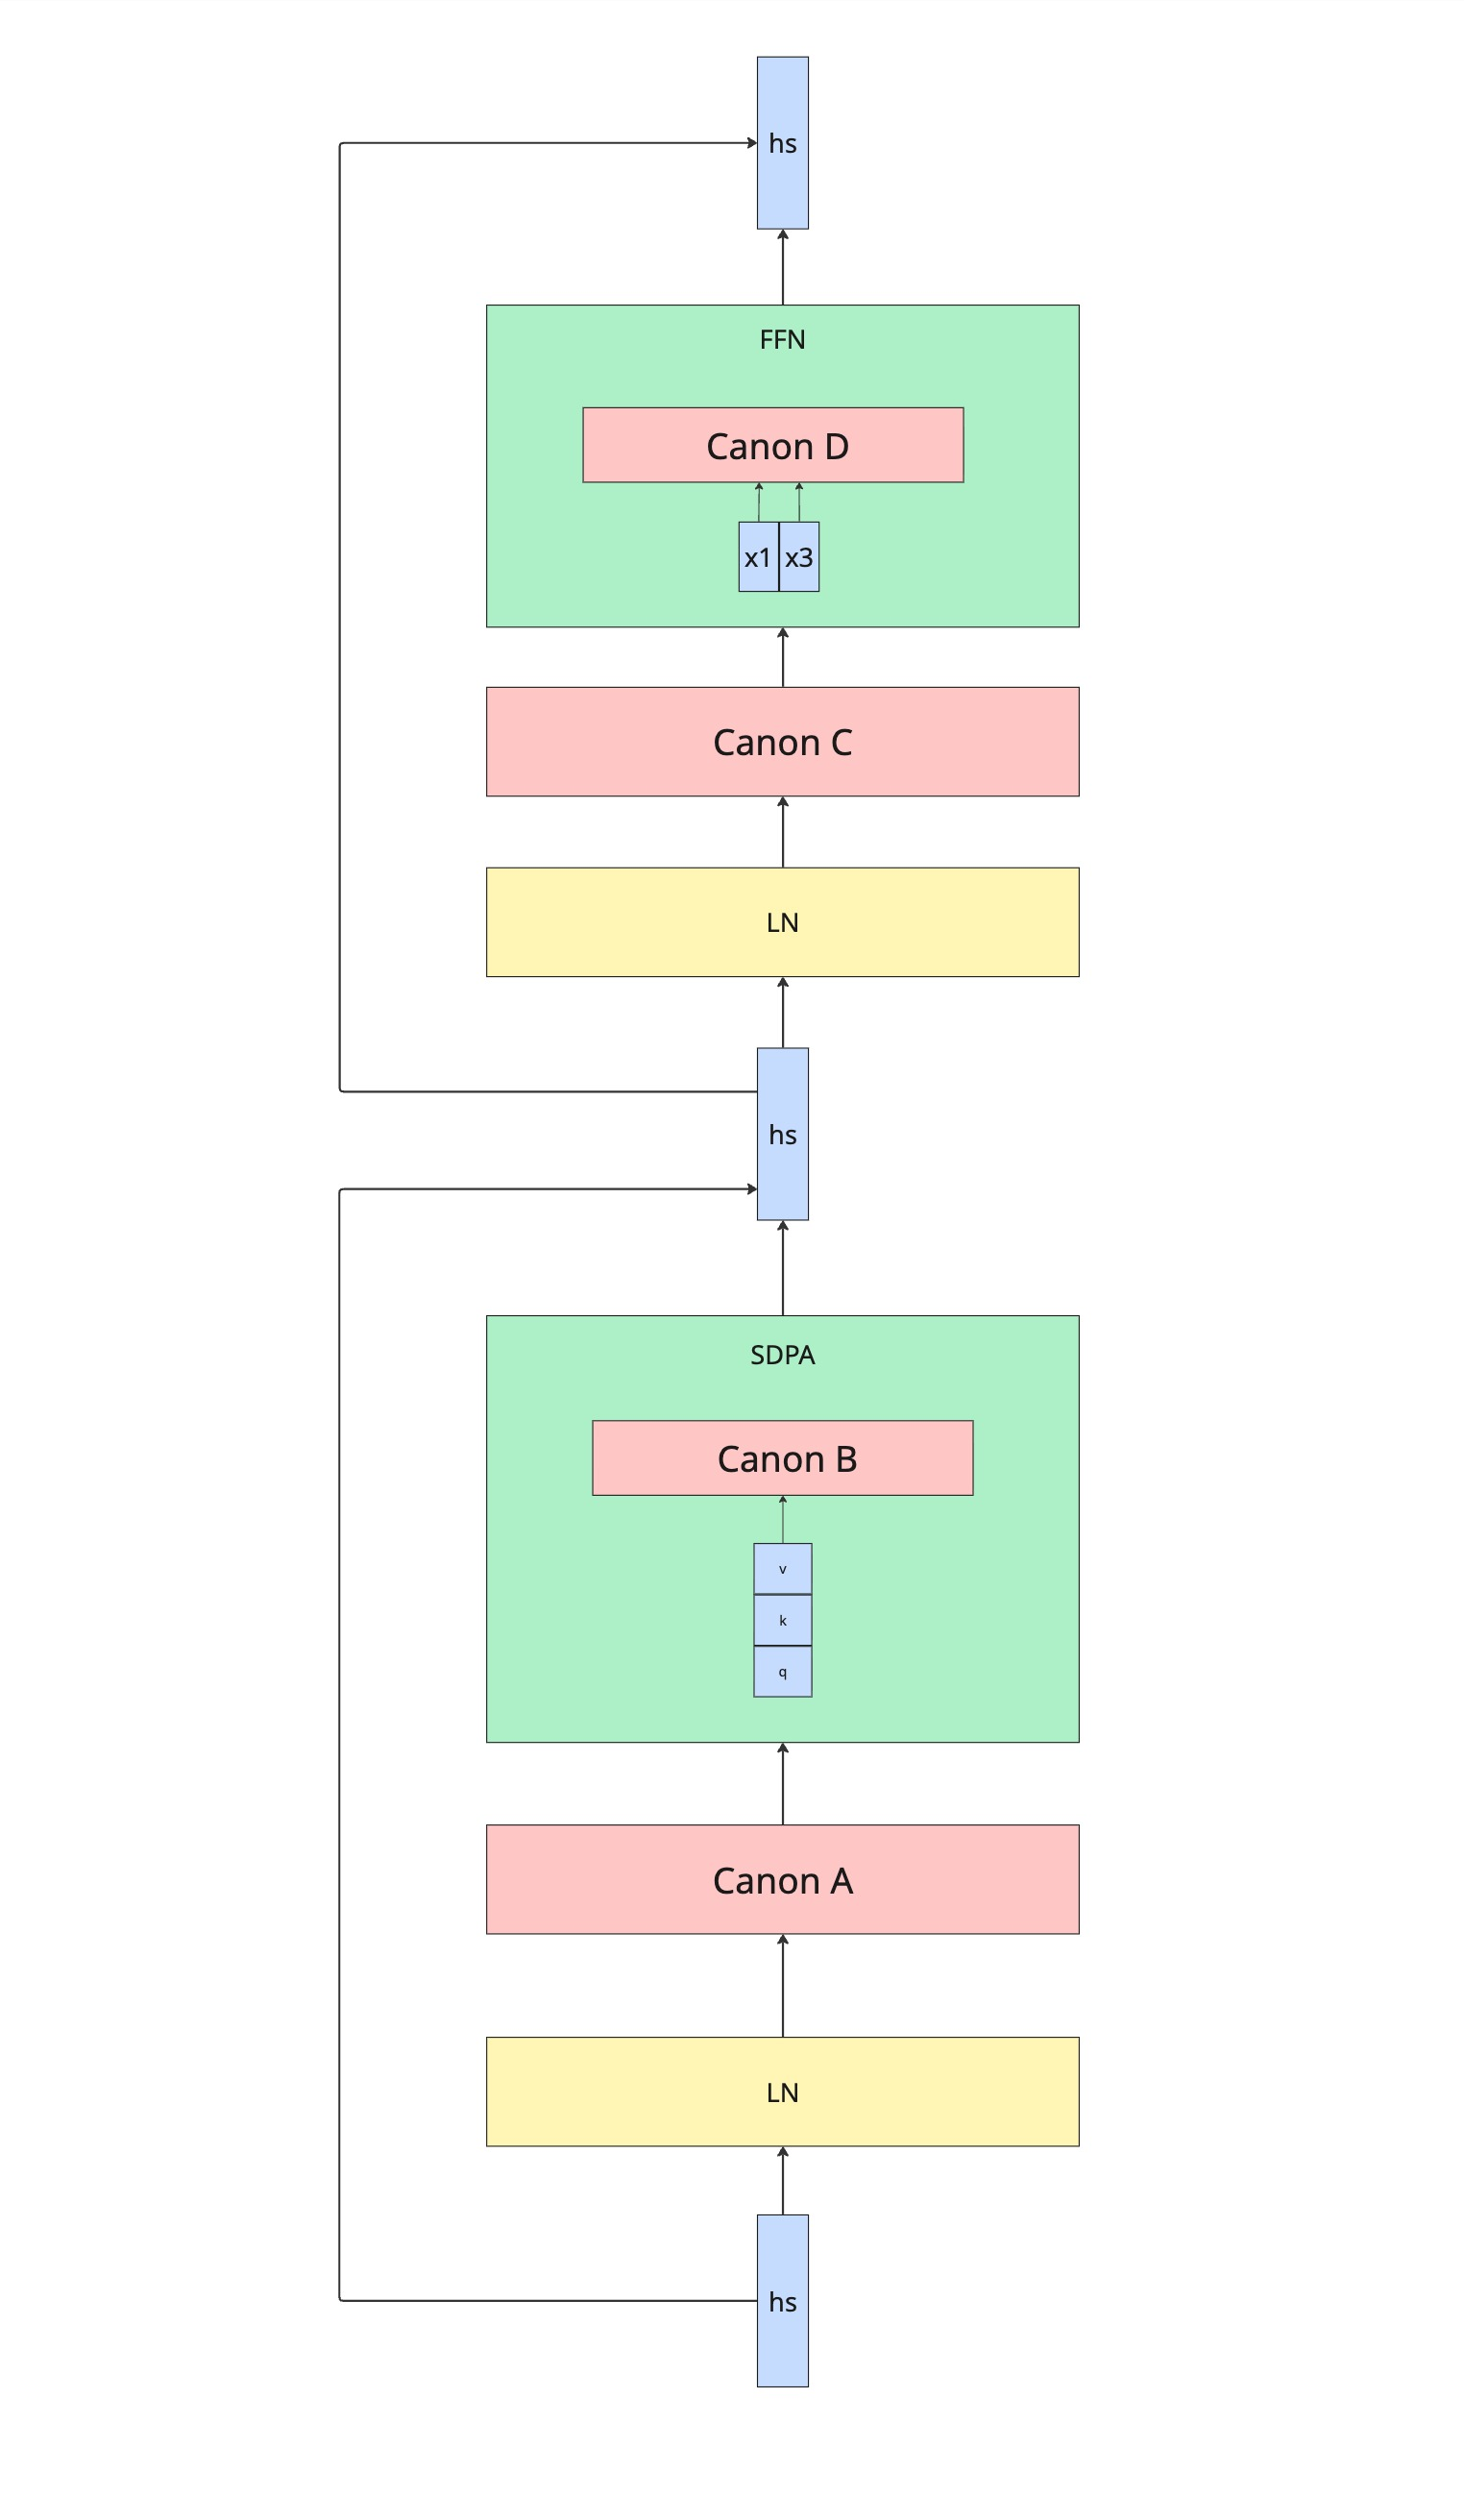
\includegraphics[width=0.5\textwidth]{canon_location_scheme.jpg}
  \caption{\textbf{Canon insertion points.} A depthwise causal convolution can be placed at
  four positions within a transformer block: pre-attention (A), post-attention (B), pre-FFN
  (C), and post-FFN (D). \Canon denotes the full A/B/C/D configuration; the baseline \Llama
  removes all four.}
  \label{fig:canon_scheme}
\end{figure}

\paragraph{Tasks and metrics.}
The benchmarks are graph-reasoning problems presented as token sequences. \Depo tests
multi-hop knowledge retrieval (following a chain of $k$ pointers), scored by hop-$k$
accuracy. BFS tests breadth-first traversal (set recall), Shortest-Path tests path-finding
(set accuracy), and ConComp tests connected-component factorization (prefix accuracy).
\Brevo tests reasoning breadth over a DAG and is excluded from the training mix because it
is too unstable to train reliably. Each task is presented in two encodings, an
edges-list and an adjacency-list form, which we treat as separate tasks. The standard
training signal is the 8-task mix: the four core tasks in both encodings.

\paragraph{Configuration.}
We train in a modified Meta Lingua framework, with the Canon convolution implemented through
the \texttt{Dao-AILab/causal-conv1d} CUDA kernel. \Canon and \Llama are matched in width,
depth, optimiser, data, and token budget. Unless stated otherwise the default model has 30M
parameters (8 layers, width 512), uses kernel size $k=4$ at all four positions, and trains
on the 8-task mix. We optimise with AdamW (learning rate $3\!\times\!10^{-4}$, cosine
schedule, $\beta_1{=}0.9$, $\beta_2{=}0.98$, $\epsilon{=}10^{-6}$) for 100k steps. For the
scaling study we train at 3M, 10M, 30M, and 100M parameters with five seeds per
(architecture, size) cell. The single metric we use for cross-architecture comparison is
the held-out language-modelling loss (\texttt{loss/out}); per-task accuracies are used for
the task-level breakdowns.

\section{Experiments}

\subsection{Reliability of Synthetic Benchmarks}
\label{sec:reliability}

A single training run is not sufficient to make reliable architectural comparisons on these
benchmarks. Text modelling is stable across seeds, but \Depo and \Brevo exhibit grokking \citep{power2022grokking}:
the loss holds a plateau before dropping sharply, and the step at which this occurs is
seed-dependent. The timing difference is large enough that a single \Canon seed can finish
above or below a single \Llama seed depending entirely on initialization. The instability is
localized: pooling five seeds per architecture at 30M, the seed-to-seed spread of the final
score concentrates almost entirely on \Depo, while every graph-search task (BFS,
Shortest-Path, ConComp) remains stable across seeds (Figure~\ref{fig:reliability}).

\begin{figure}[t]
  \centering
  \begin{subfigure}{0.49\textwidth}
    
\includegraphics[width=\linewidth]{text_stable.png}
    \caption{Text modelling: seeds nearly identical.}
  \end{subfigure}\hfill
  \begin{subfigure}{0.49\textwidth}
    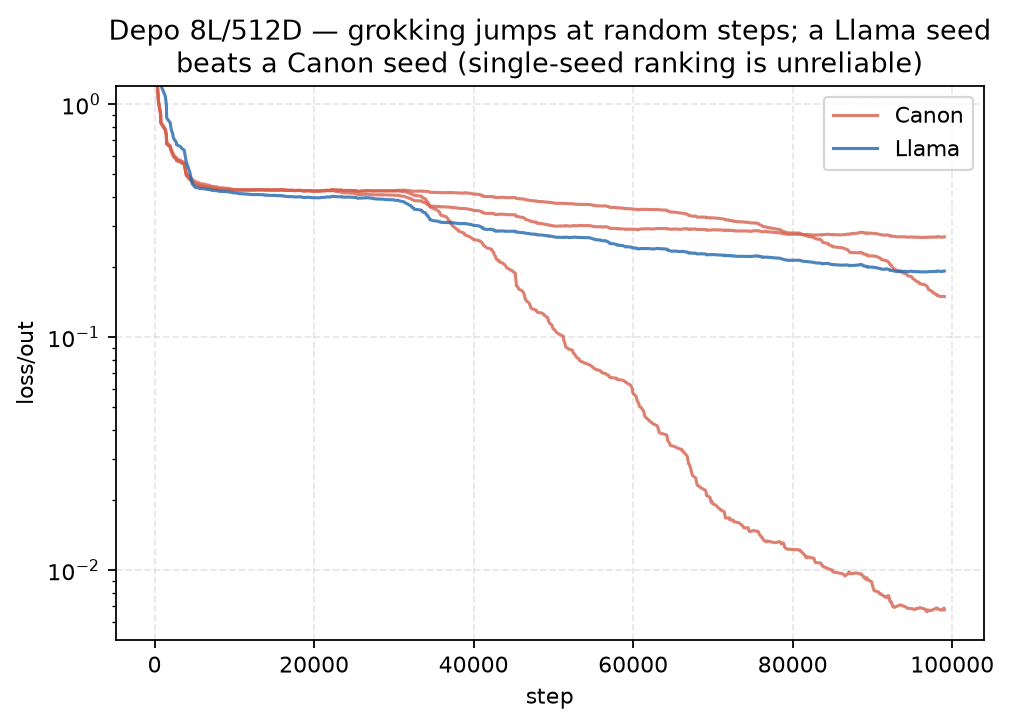
\includegraphics[width=\linewidth]{depo_grokking.png}
    \caption{\Depo: grokking jumps at random steps.}
  \end{subfigure}

  \vspace{0.6em}
  \begin{subfigure}{0.49\textwidth}
    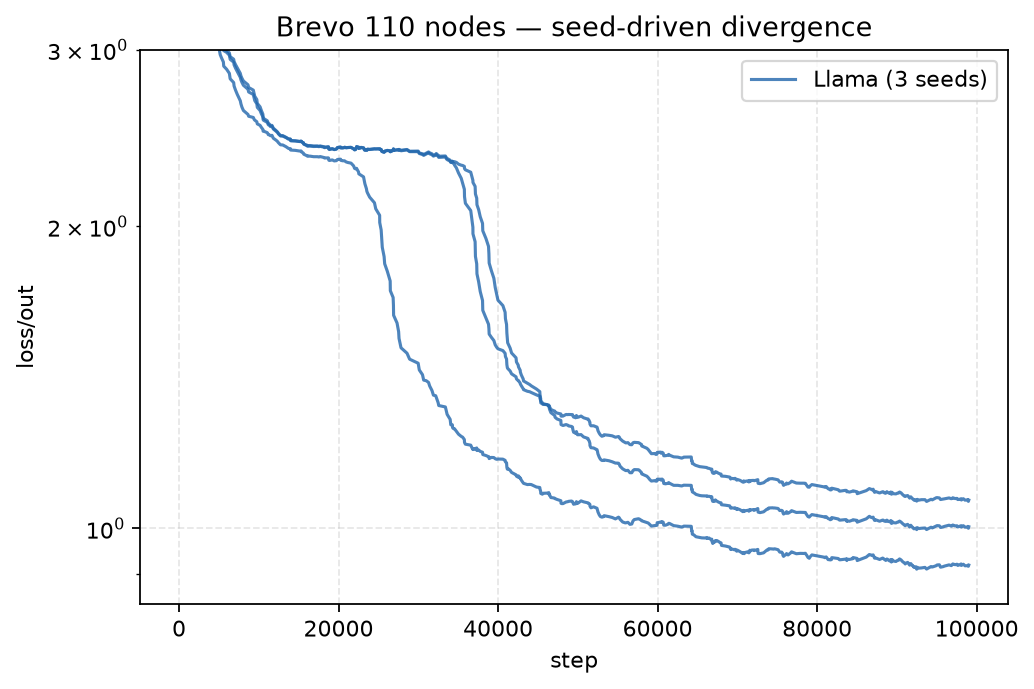
\includegraphics[width=\linewidth]{brevo.png}
    \caption{\Brevo: seed-driven divergence.}
  \end{subfigure}\hfill
  \begin{subfigure}{0.49\textwidth}
    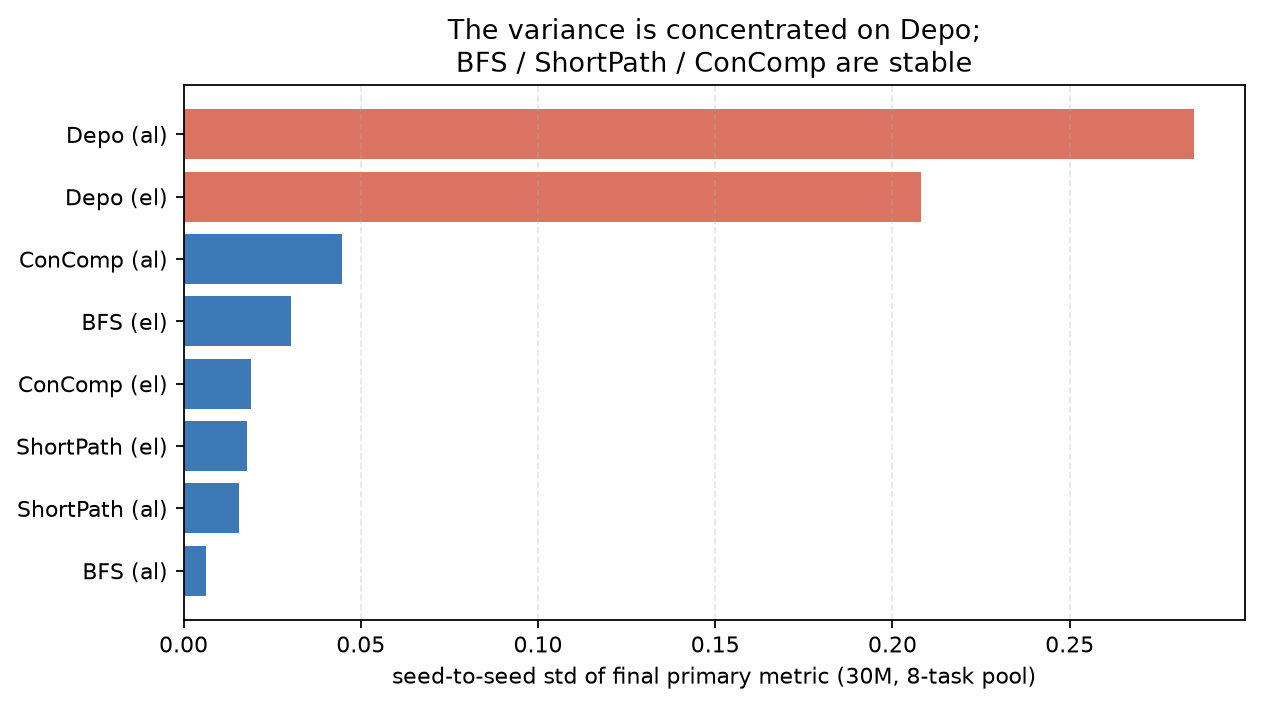
\includegraphics[width=\linewidth]{task_noise.png}
    \caption{Variance is concentrated on \Depo.}
  \end{subfigure}
  \caption{\textbf{Benchmark reliability varies by task.} Text modelling is stable across
  seeds; \Depo and \Brevo grok at a seed-dependent step, making single-run rankings
  unreliable. Seed-to-seed variance concentrates on \Depo; all graph-search tasks are
  stable.}
  \label{fig:reliability}
\end{figure}

Any ranking claim on these benchmarks must therefore average over seeds, and since the gap
between architectures can change with model size, over several scales.

The volatility of \Depo does not mean the depth-of-reasoning skill it probes is itself
unmeasurable. Across the 40 scaling runs (both architectures $\times$ four scales $\times$
five seeds), of all the stable graph-search tasks ConComp is the one whose accuracy tracks
\Depo grokking most strongly: whether a run has grokked \Depo is most predictive of its
ConComp score. ConComp exercises the same global, multi-step composition over the graph but
without the sharp grokking transition, so it is a more stable proxy for the same
depth-of-reasoning ability.

\subsection{Canon Consistently Improves Performance Across Seeds and Scales}
\label{sec:scaling}

Averaged over five seeds per point, \Canon achieves lower loss than \Llama at every scale
from 3M to 100M parameters (Figure~\ref{fig:scaling}). The gap is largest for small models
and narrows with scale, but the ordering never reverses. At 30M the gain is concentrated on
\Depo, where \Canon adds a large accuracy margin on both encodings; improvements on ConComp
are minor, and BFS and Shortest-Path are already solved by both architectures. Notably,
\Canon's benefit is largest on the same volatile, grokking-prone task identified in
Section~\ref{sec:reliability}, which is why single-seed evaluations of it are so easy to
misread: grokking, seed variance, and architectural benefit all coincide on multi-hop
retrieval.

\begin{figure}[t]
  \centering
  \begin{subfigure}{0.40\textwidth}
    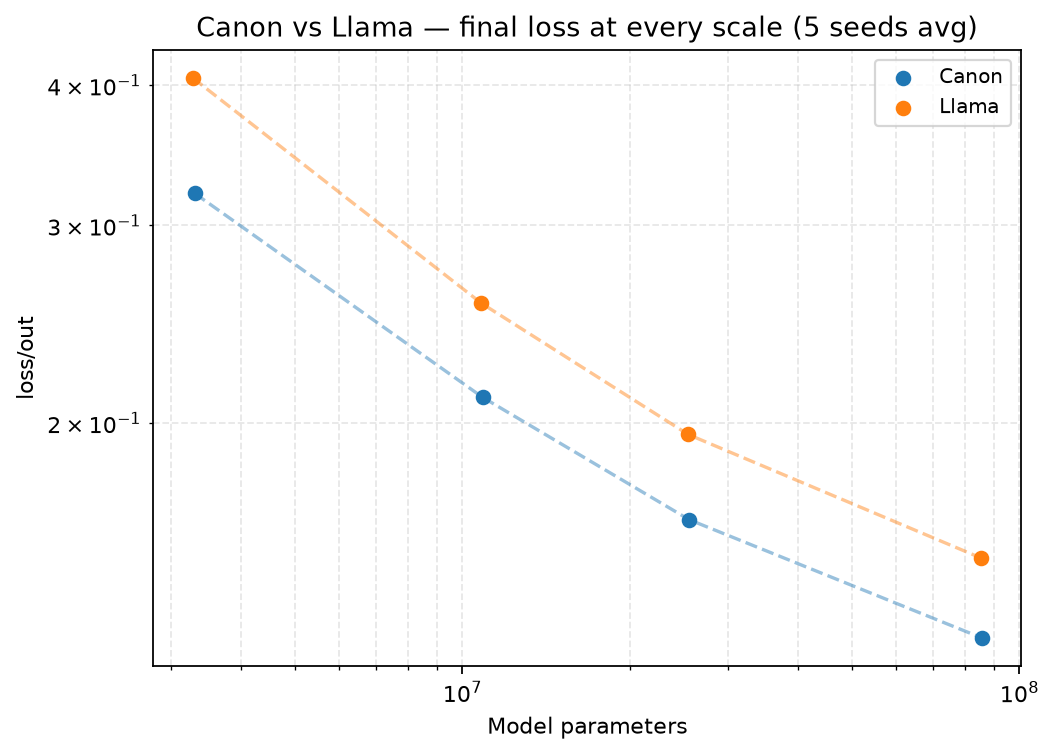
\includegraphics[width=\linewidth]{scaling.png}
    \caption{Loss vs.\ parameters (5 seeds avg).}
  \end{subfigure}\hfill
  \begin{subfigure}{0.58\textwidth}
    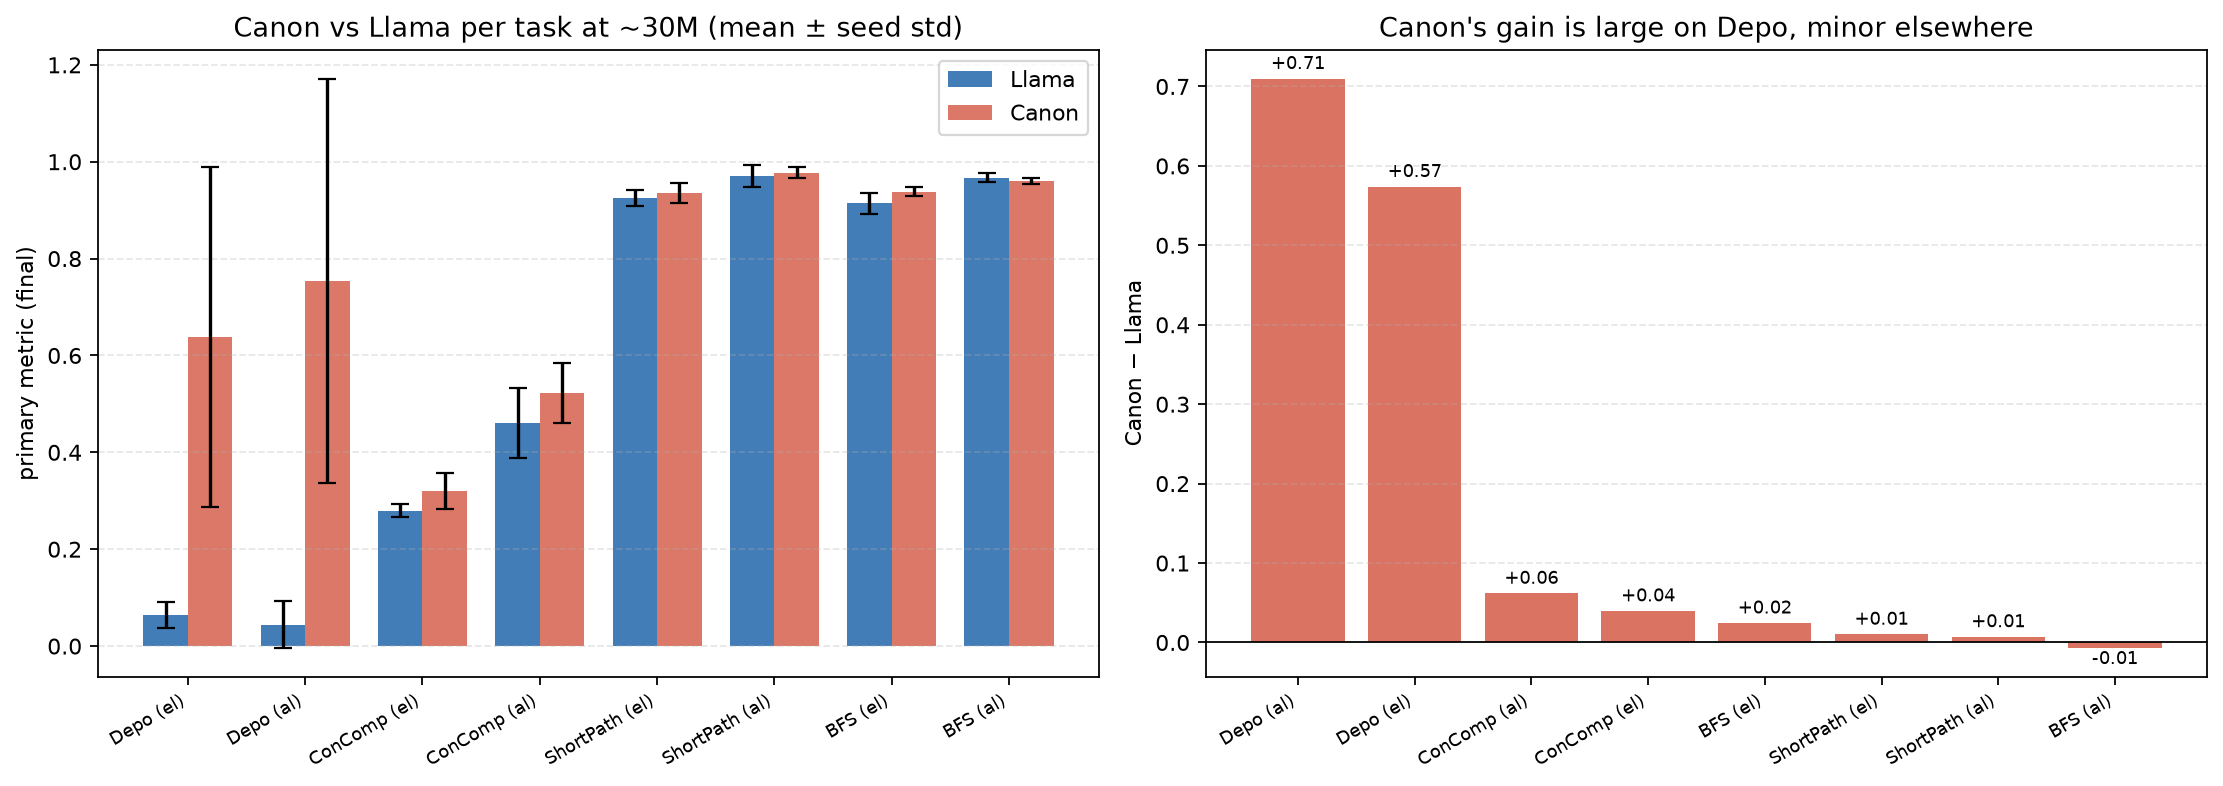
\includegraphics[width=\linewidth]{task_breakdown.png}
    \caption{Per-task breakdown at 30M.}
  \end{subfigure}
  \caption{\textbf{\Canon outperforms \Llama at every scale when averaging over seeds.}
  The gap is largest for small models and narrows with scale. At 30M the gain is
  concentrated on \Depo; improvements on other tasks are minor or absent.}
  \label{fig:scaling}
\end{figure}

\subsection{Canon Substitutes for Model Depth}
\label{sec:depth}

The scaling sweep grows the model by widening it. A complementary question is how
the two architectures respond to \emph{depth}. We train a param-matched depth sweep at
roughly 85M parameters, varying the number of layers while shrinking the width to hold the
parameter count fixed (10 layers at width 832, 12 at 768, 14 at 704), with both
architectures trained on the 8-task mix.

\Llama improves steadily as it is made deeper: its loss falls from $0.181$ at 10 layers to
$0.103$ at 14 (Figure~\ref{fig:depth}, left). The improvement is concentrated on multi-hop
retrieval: a 10-layer \Llama is at the floor on \Depo (hop-4 accuracy $0.16$) and only
solves the task once it has 14 layers ($0.93$). Depth is what lets the baseline acquire the
multi-hop capability.

\Canon reaches the same capability several layers shallower. A 10-layer \Canon model already
attains \Depo accuracy $0.86$ and a lower aggregate loss ($0.141$) than a 12-layer \Llama,
and a 12-layer \Canon model ($0.127$) is the strongest configuration of either architecture,
matching a 14-layer \Llama on \Depo (Figure~\ref{fig:depth}, right). The cross-token mixing
Canon adds supplies what \Llama otherwise obtains only by stacking more layers, which is
consistent with the gain being largest on the task that most requires composing information
across positions. The depth points use a single seed per configuration and \Depo is
grokking-prone (Section~\ref{sec:reliability}), so we read the trend rather than the
individual points; the direction is consistent across both depths at which \Canon is
available.

\begin{figure}[t]
  \centering
  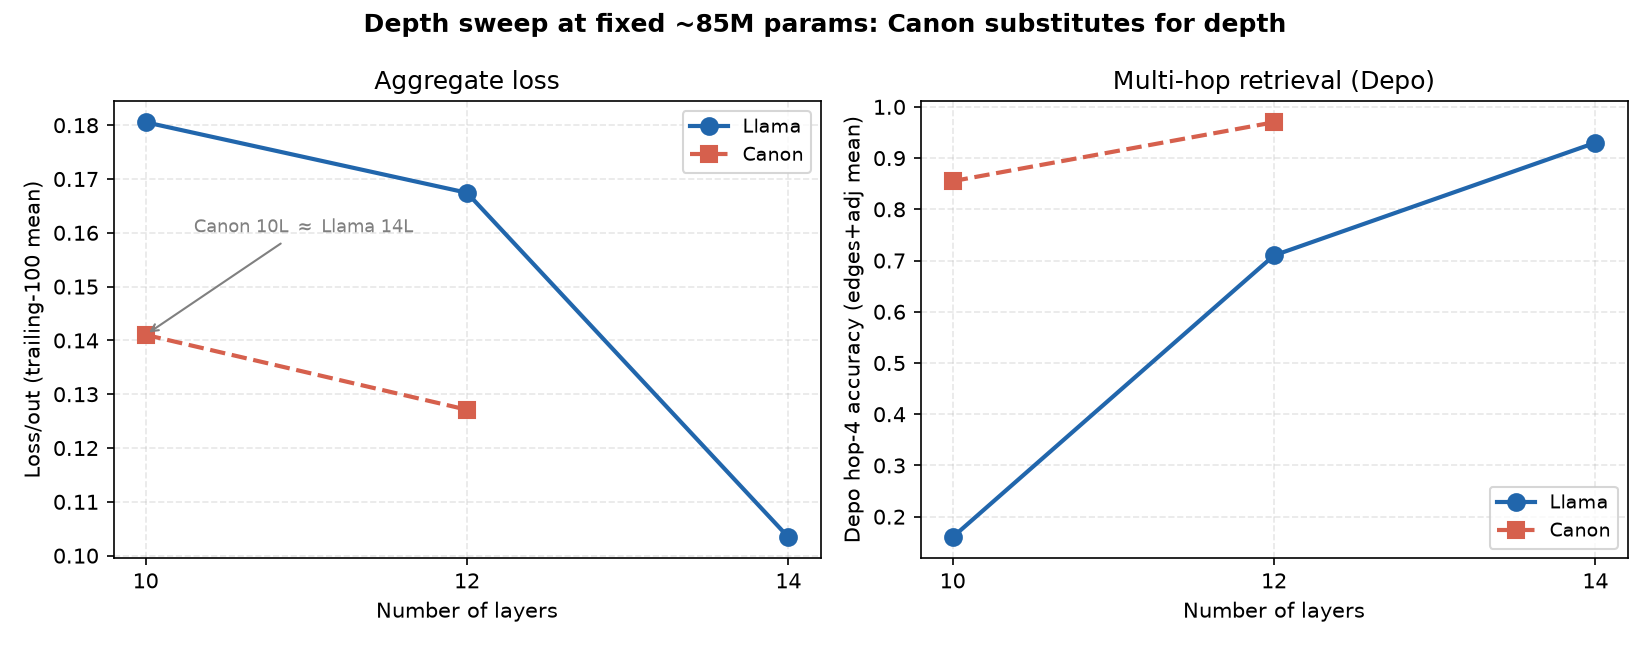
\includegraphics[width=0.92\textwidth]{depth_85m.png}
  \caption{\textbf{\Canon substitutes for model depth (param-matched, $\sim$85M).} \Llama
  improves with depth, acquiring multi-hop retrieval (\Depo) only at 14 layers; \Canon
  reaches comparable performance several layers shallower. \Canon at 10 layers matches a
  14-layer \Llama on \Depo, and \Canon at 12 layers is the strongest model overall.}
  \label{fig:depth}
\end{figure}

\subsection{From Synthetic Benchmarks to Text: Where Mechanism Can Be Studied}
\label{sec:mechanism}

The seed-averaged ranking settles whether \Canon helps but not why. A natural next step is
to read \Canon's mechanism off the synthetic suite directly: even if the final score on a
grokking task is seed-unreliable (Section~\ref{sec:reliability}), the model's internal
training dynamics might be more stable. We find this hope is only partly borne out, which
leads us to study mechanism on text instead.

\paragraph{Some coarse signatures reproduce.}
The deep/shallow gradient ratio is seed-stable on the synthetic tasks: where the final \Depo
score swings seed to seed, the trajectory of this ratio is reproducible, with the \Canon
seeds held low and tightly bundled and the \Llama seeds drifting upward, the two bundles
never crossing (Figure~\ref{fig:mech_hope}, left). This synthetic signature also agrees
qualitatively with the same measurement on text (Figure~\ref{fig:mech_hope}, right), which
is encouraging: a coarse statistic about gradient flow transfers between the two regimes.

\begin{figure}[t]
  \centering
  \begin{subfigure}{0.49\textwidth}
    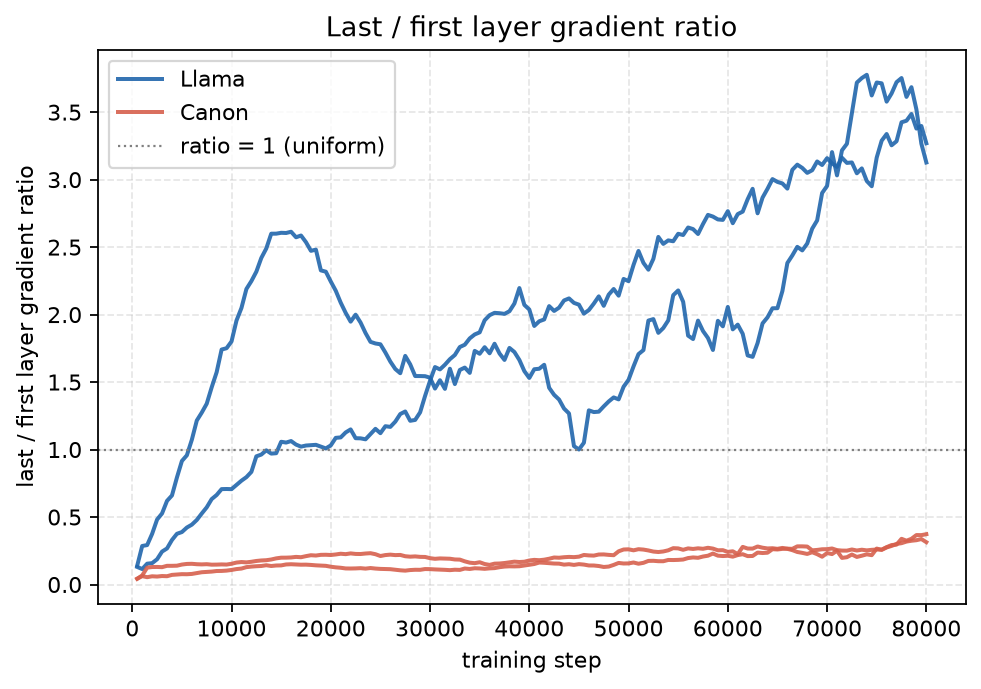
\includegraphics[width=\linewidth]{grad_ratio_seeds.png}
    \caption{Synthetic, one line per seed.}
  \end{subfigure}\hfill
  \begin{subfigure}{0.49\textwidth}
    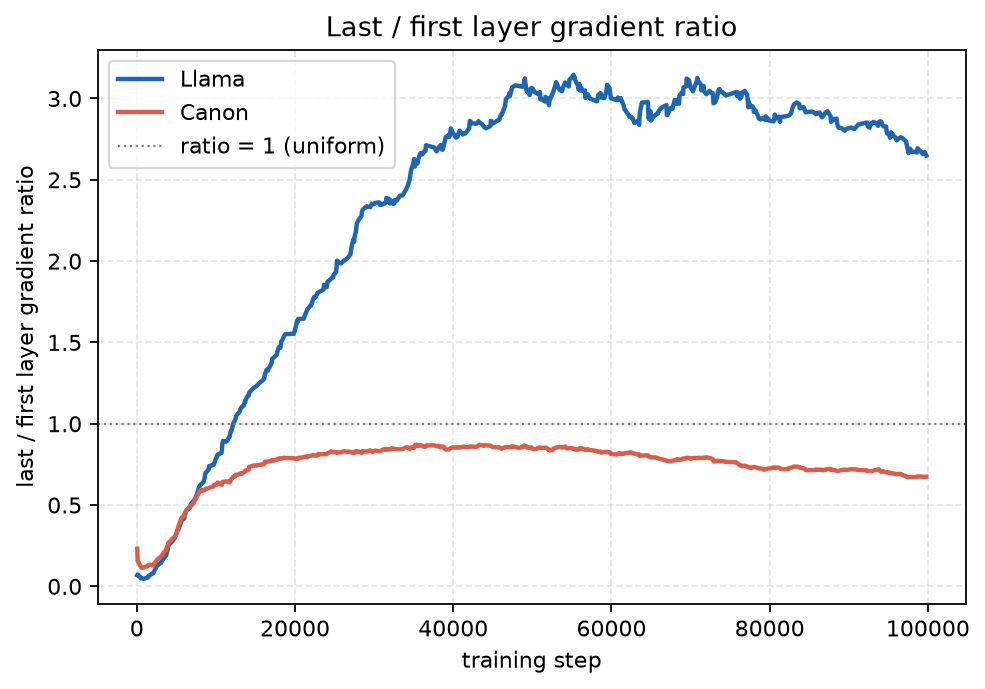
\includegraphics[width=\linewidth]{grad_ratio.png}
    \caption{Text.}
  \end{subfigure}
  \caption{\textbf{A coarse signature that does transfer.} Deep/shallow gradient ratio over
  training. On the synthetic tasks (left) it is seed-stable, with the \Canon and \Llama seeds
  forming two non-overlapping bundles even though the final \Depo score varies seed to seed, and
  it agrees qualitatively with the same measurement on text (right).}
  \label{fig:mech_hope}
\end{figure}

\paragraph{The informative signatures do not.}
The more detailed mechanistic signatures, however, do not transfer. The per-layer gradient
profile and the residual-stream RMS ratio look qualitatively different on the synthetic
tasks than on text (Figure~\ref{fig:synth_vs_text}): the synthetic dynamics are dominated by
the grokking transition and lack the clean across-depth structure visible in text. Drawing
mechanistic conclusions from the synthetic runs is therefore unreliable. We accordingly study
\Canon's mechanism on text, where the dynamics are stable and reproducible, and reserve the
synthetic suite for the reliability and ranking results above.

\begin{figure}[t]
  \centering
  \begin{subfigure}{0.24\textwidth}
    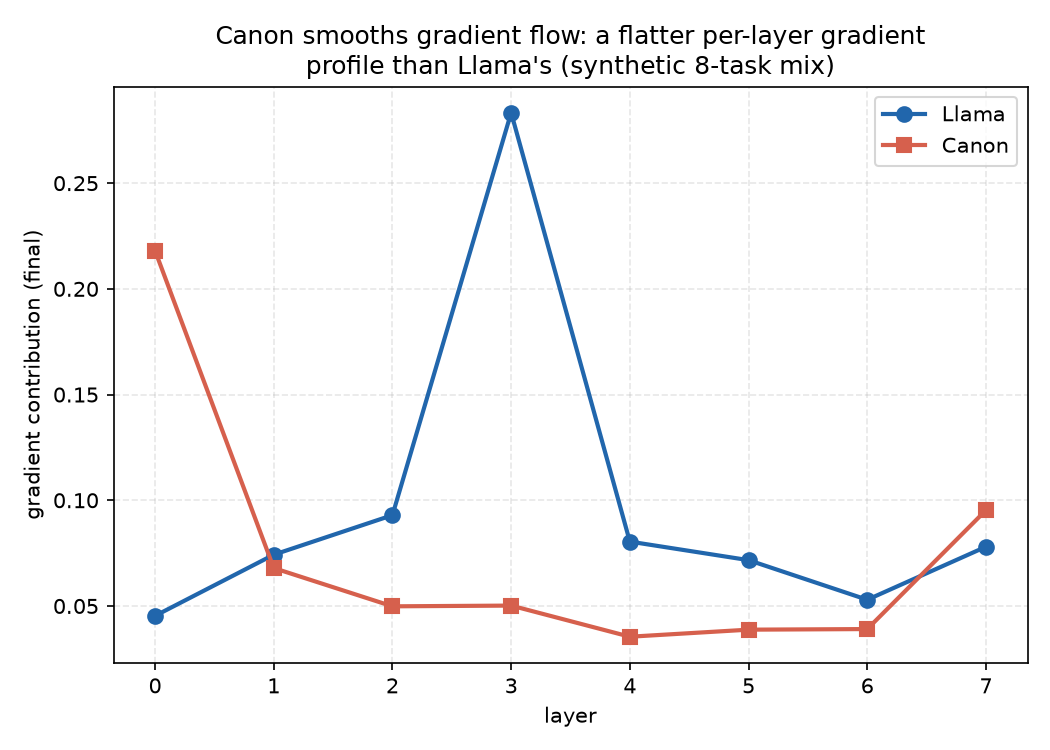
\includegraphics[width=\linewidth]{grad_profile_synth.png}
    \caption{Profile, synthetic.}
  \end{subfigure}\hfill
  \begin{subfigure}{0.24\textwidth}
    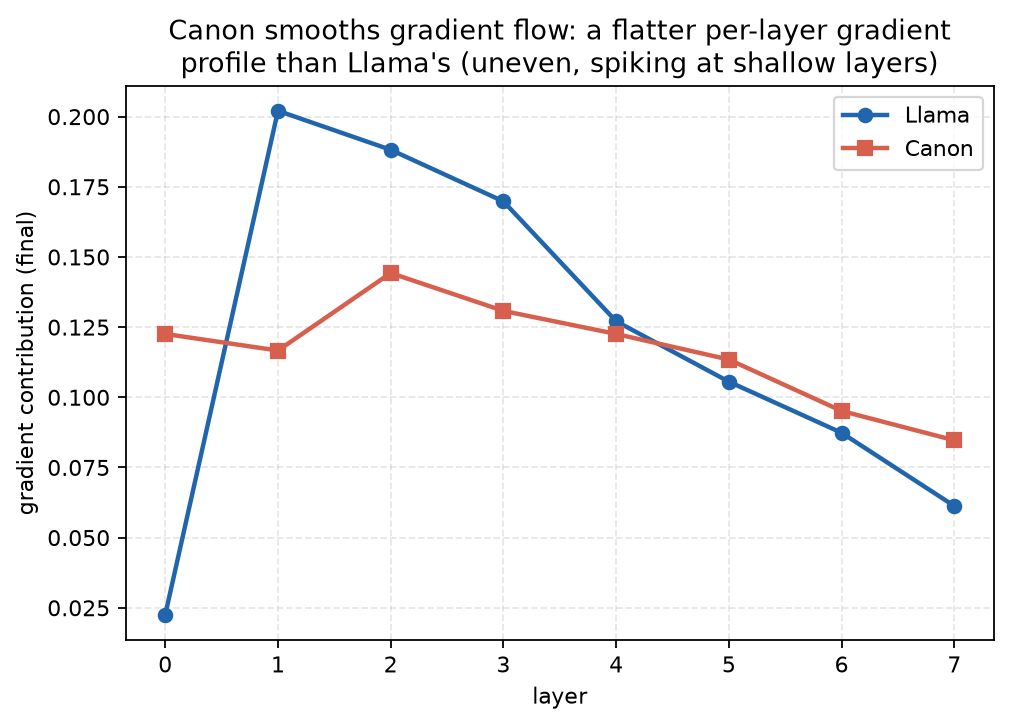
\includegraphics[width=\linewidth]{grad_profile.png}
    \caption{Profile, text.}
  \end{subfigure}\hfill
  \begin{subfigure}{0.24\textwidth}
    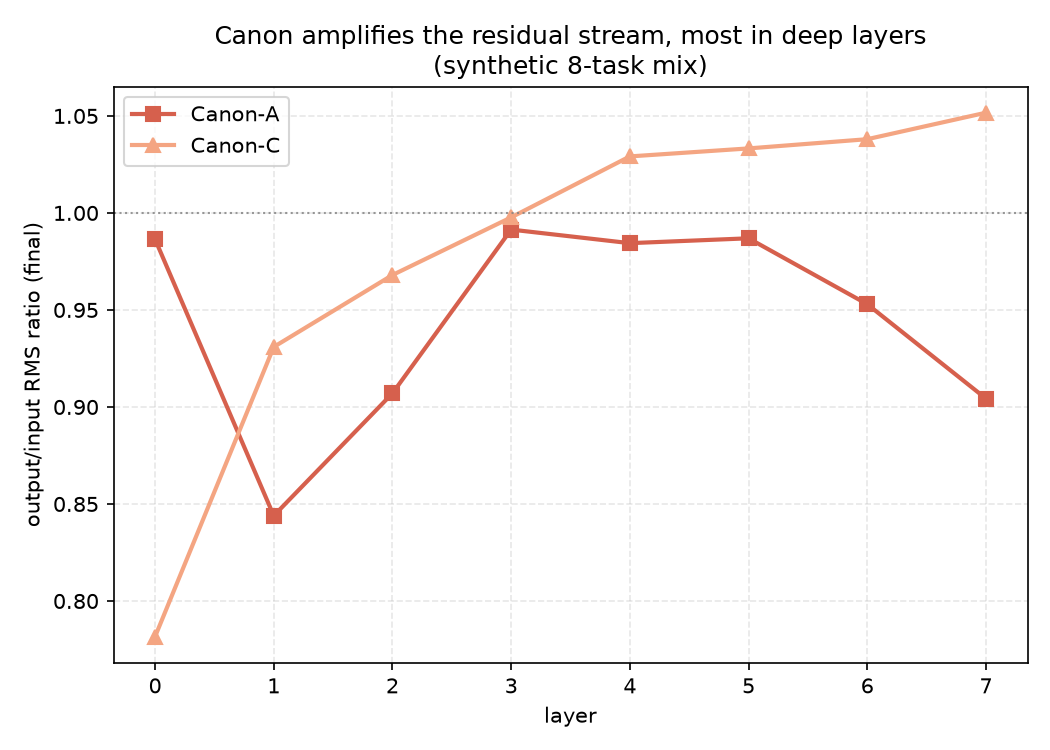
\includegraphics[width=\linewidth]{rms_ratio_synth.png}
    \caption{RMS ratio, synthetic.}
  \end{subfigure}\hfill
  \begin{subfigure}{0.24\textwidth}
    
\includegraphics[width=\linewidth]{rms_ratio.png}
    \caption{RMS ratio, text.}
  \end{subfigure}
  \caption{\textbf{The informative dynamics do not reproduce on the benchmarks.} The
  per-layer gradient profile and the residual-stream RMS ratio differ qualitatively between
  the synthetic tasks and text. Because the synthetic dynamics are dominated by grokking,
  we study \Canon's mechanism on text.}
  \label{fig:synth_vs_text}
\end{figure}

\subsubsection{Across-Layer Training Dynamics on Text}

On text, \Canon leaves two reproducible across-layer signatures
(Figure~\ref{fig:synth_vs_text}, right panels). First, \emph{gradient smoothing}: \Llama
develops a strong deep-layer gradient dominance over training, with deep layers increasingly
dominating the gradient signal, whereas \Canon suppresses this effect and distributes the
per-layer gradient profile more evenly across depth. Second, \emph{representation upscaling}:
the \Canon convolution amplifies the residual stream, with the convolution output/input RMS
ratio exceeding one most strongly in the deep layers near the language-modelling head. Both
changes resemble the effect of scaling the model up, and are consistent with the gain being
concentrated on the depth-of-reasoning tasks.

\subsubsection{Cross-Token Mixing Is the Essential Ingredient}

Setting $k{=}1$ removes cross-token mixing while preserving all other \Canon parameters;
this configuration performs \emph{worse} than the \Llama baseline, and loss improves
monotonically as $k$ increases from 2 to 6 (Figure~\ref{fig:flow}). Cross-token mixing is
the necessary ingredient, not the additional parameters. The learned weights place more mass
on farther-back shifts than on the current token from the first checkpoint, and the mixing
is strongest in the early layers (lowest output/input cosine similarity). \Canon is therefore
structurally biased toward integrating context from earlier tokens, a property present from
initialisation rather than acquired gradually.

\begin{figure}[t]
  \centering
  \begin{subfigure}{0.33\textwidth}
    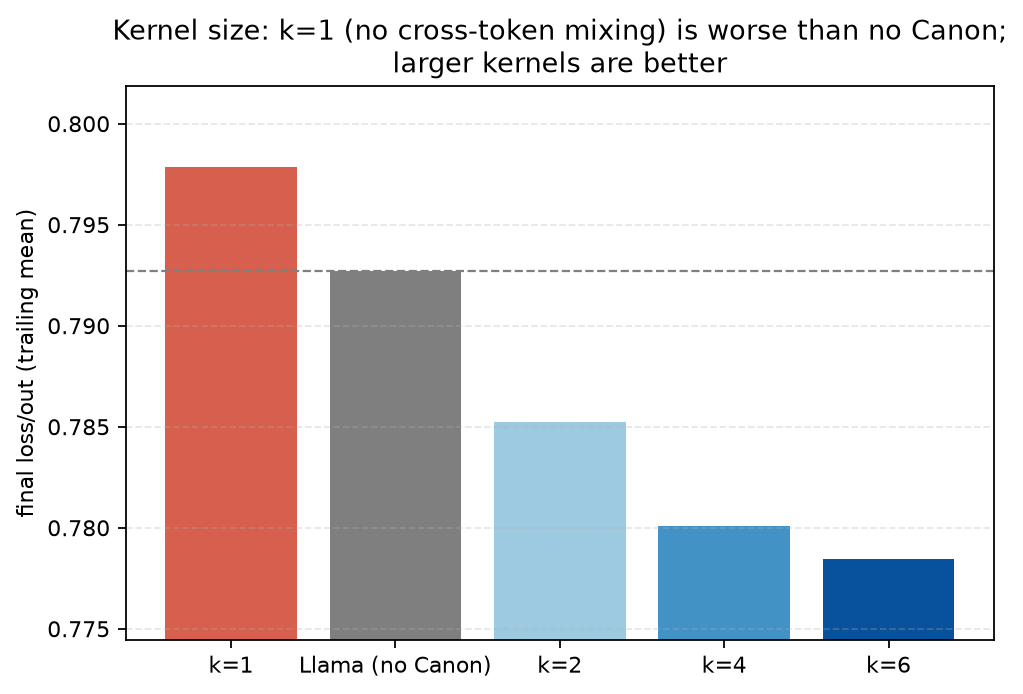
\includegraphics[width=\linewidth]{kernel.png}
    \caption{$k{=}1$ (no mixing) is worse than baseline.}
  \end{subfigure}\hfill
  \begin{subfigure}{0.33\textwidth}
    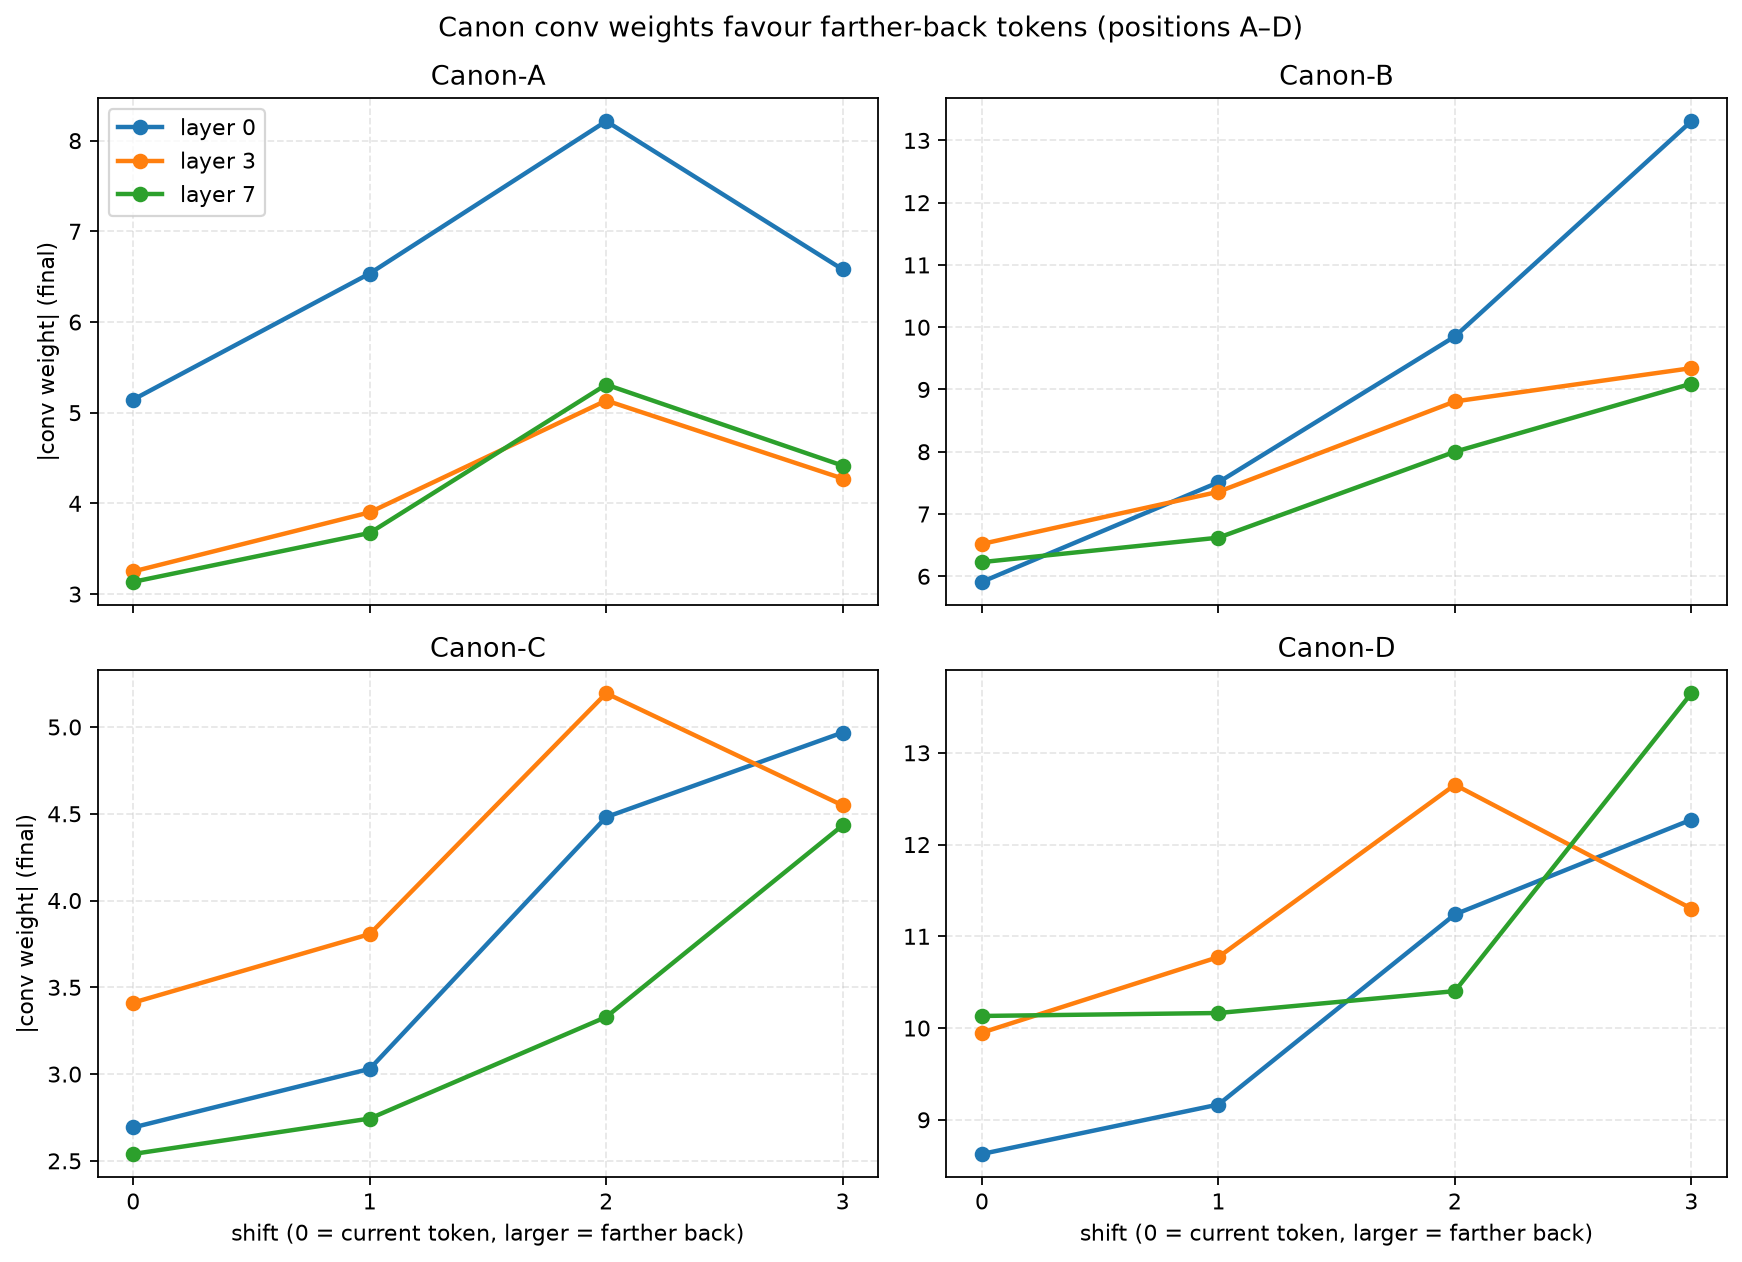
\includegraphics[width=\linewidth]{canon_weights.png}
    \caption{Weights favour farther-back tokens.}
  \end{subfigure}\hfill
  \begin{subfigure}{0.33\textwidth}
    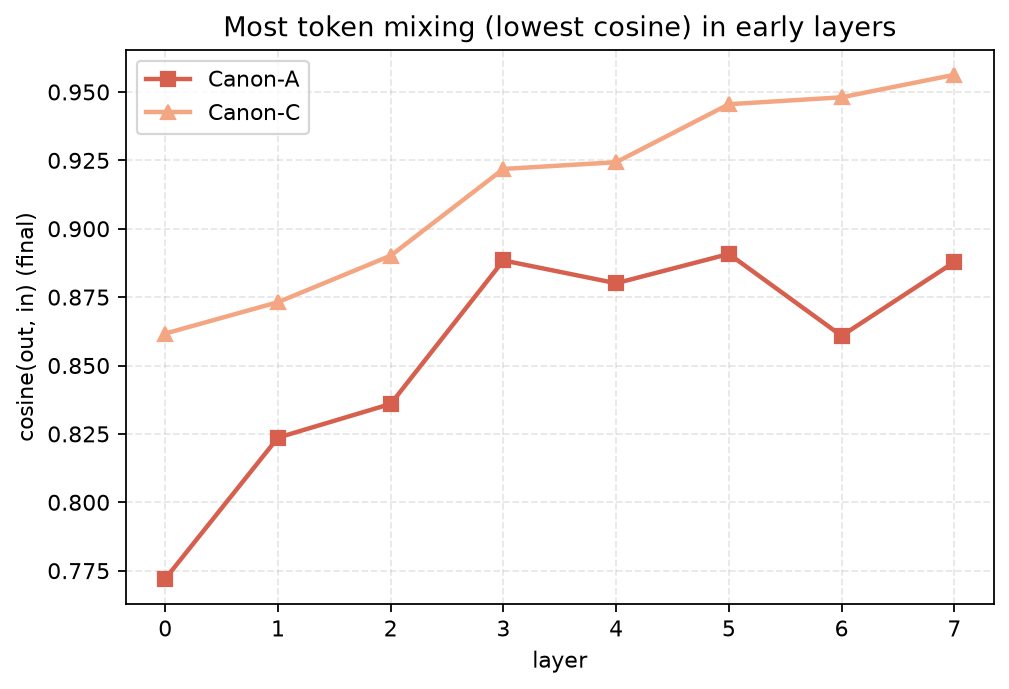
\includegraphics[width=\linewidth]{cos_sim.png}
    \caption{Most mixing in early layers.}
  \end{subfigure}
  \caption{\textbf{Cross-token mixing is the necessary ingredient.} $k{=}1$ (no mixing)
  performs worse than the baseline; loss improves monotonically with kernel size. The
  learned weights favour farther-back tokens from initialisation, with the strongest
  mixing in early layers.}
  \label{fig:flow}
\end{figure}

\subsection{Recommended Configuration}
\label{sec:ablations}

Having established that the mechanism is best studied on text, we ablate on text the two
remaining design choices that are easy to vary: where the convolution is inserted and how its
weights are initialised. Together with the kernel-size sweep above, these ablations yield a
recommended configuration.

\paragraph{Insertion positions: A and C are sufficient.}
A transformer block offers four insertion points (A through D, as described in
Section~\ref{sec:background}).
The full A/B/C/D configuration is not necessary: placing convolutions only at positions
A (pre-attention) and C (pre-FFN) recovers essentially the entire gain
(Figure~\ref{fig:ablations}, left). The B and D positions (post-attention and
post-FFN) contribute negligibly and can be dropped without loss. This makes \Canon a
minimal, two-point intervention on the standard transformer block.

\paragraph{Initialisation: the benefit is robust.}
All initialisation schemes tested beat the \Llama baseline, including zero initialisation
(Figure~\ref{fig:ablations}, right). Zero-init starts as a no-op and recovers the
benefit through learning; the $1/k$ constant-variance scheme (\texttt{const\_var\_sqrt})
is best but the gap over other schemes is small. The structural benefit of the convolution
does not depend on the initialisation choice.

\begin{figure}[t]
  \centering
  \begin{subfigure}{0.49\textwidth}
    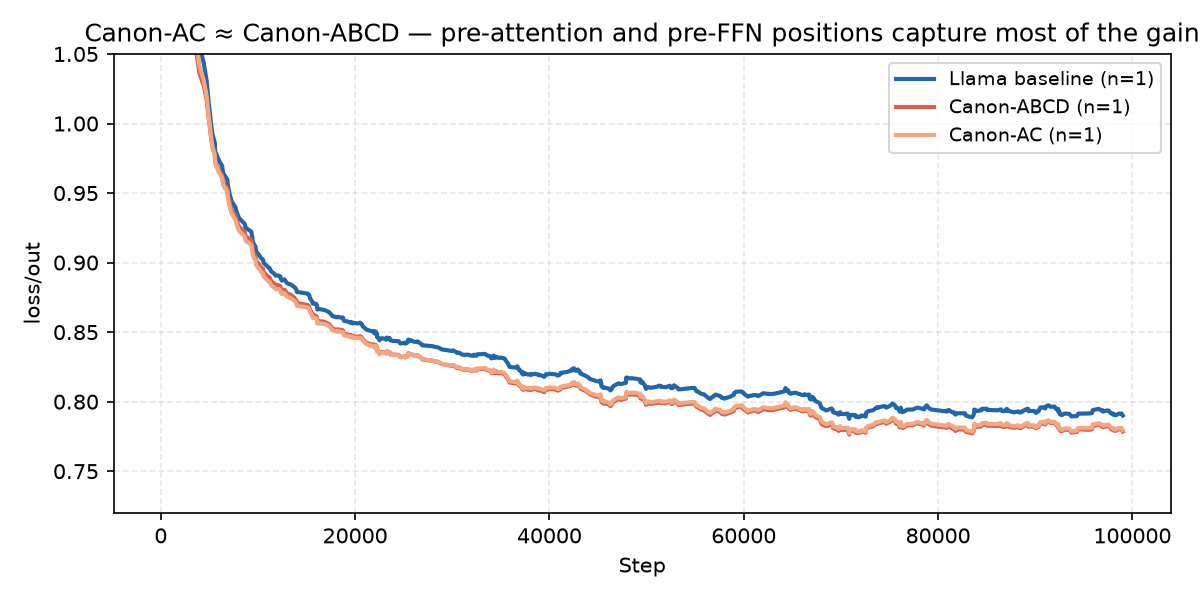
\includegraphics[width=\linewidth]{ac_vs_abcd.png}
    \caption{Canon-AC matches Canon-ABCD.}
  \end{subfigure}\hfill
  \begin{subfigure}{0.49\textwidth}
    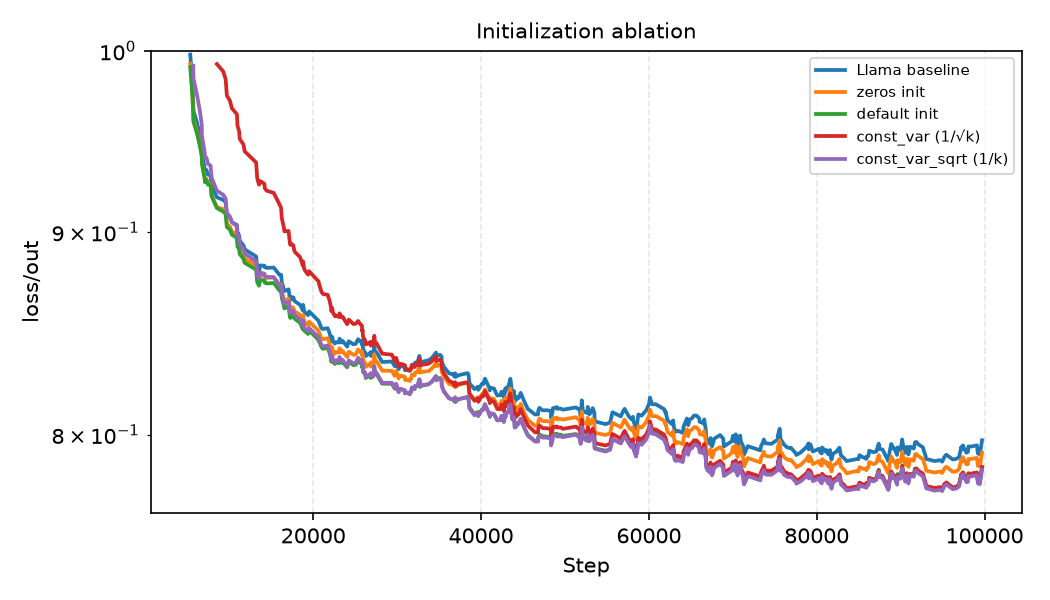
\includegraphics[width=\linewidth]{initialization.png}
    \caption{All init schemes beat the baseline.}
  \end{subfigure}
  \caption{\textbf{\Canon configuration ablations (text).} Positions A and C (pre-attention and
  pre-FFN) capture the full gain; B and D are droppable. All initialisation schemes
  outperform the \Llama baseline, including zero initialisation; the benefit is
  structurally inherent to the convolution, not to the choice of starting weights.}
  \label{fig:ablations}
\end{figure}

\paragraph{Recommendation.}
The ablations converge on a single recommended setting: \textbf{\Canon-AC with kernel size
$k{=}4$ and the default initialisation}. Positions A and C recover the full gain of the
four-point configuration at half the convolutions; $k{=}4$ saturates the kernel-size benefit
(larger kernels add little, while $k{=}1$ is worse than no \Canon at all); and the benefit is
robust to the initialisation scheme.

\section{Discussion}

\paragraph{On Canon.}
\Canon consistently outperforms the \Llama baseline at every scale tested, with the gain
concentrated on multi-hop retrieval (\Depo). The causal convolution provides cross-token
mixing that is structurally biased toward long-range context from initialisation: removing
it ($k{=}1$) degrades performance below the baseline, confirming mixing is the essential
structural ingredient. \Canon also produces reproducible across-layer signatures (gradient
redistribution and deep-layer representation amplification) that are consistent across
seeds and reflect how the convolution reshapes the model's internal computation.

\paragraph{Methodological lesson.}
These benchmarks mislead when read one seed at a time, because grokking makes a single training
curve on the volatile tasks largely a function of the seed. The fix for ranking claims is
to average over seeds and sweep scale; it is simple but not optional, and which tasks
demand it is not obvious a priori. The benchmarks are also limited as a tool for mechanistic
interpretation: while coarse training signatures such as the deep/shallow gradient ratio
reproduce across seeds and agree with text, the more informative dynamics (the per-layer
gradient profile and residual-stream scaling) are dominated by the grokking transition and do
not match text training. Mechanistic conclusions are therefore more reliably drawn on text,
with the synthetic suite used for reliability-aware ranking rather than as the object of
mechanistic study.

\paragraph{Limitations and future work.}
Our mechanistic evidence is observational: the signatures we document are descriptive and
do not establish causal direction. Direct interventions (frozen or surgically modified
convolution weights, or targeted gradient-flow modifications) remain future work and would
help pin down the mechanisms more precisely. We also leave the dependence on encoding
(edges-list versus adjacency-list) unexplained. Finally, the suite we study is a specific
one; whether the reliable/unreliable split we document generalises to other synthetic
benchmark families is an open question.


\bibliographystyle{abbrvnat}
\bibliography{references}

\end{document}
